\documentclass[12pt]{article}
\usepackage{fullpage}
\usepackage{tikz}
\usepackage{rotating}
\begin{document}
\begin{turn}{90}
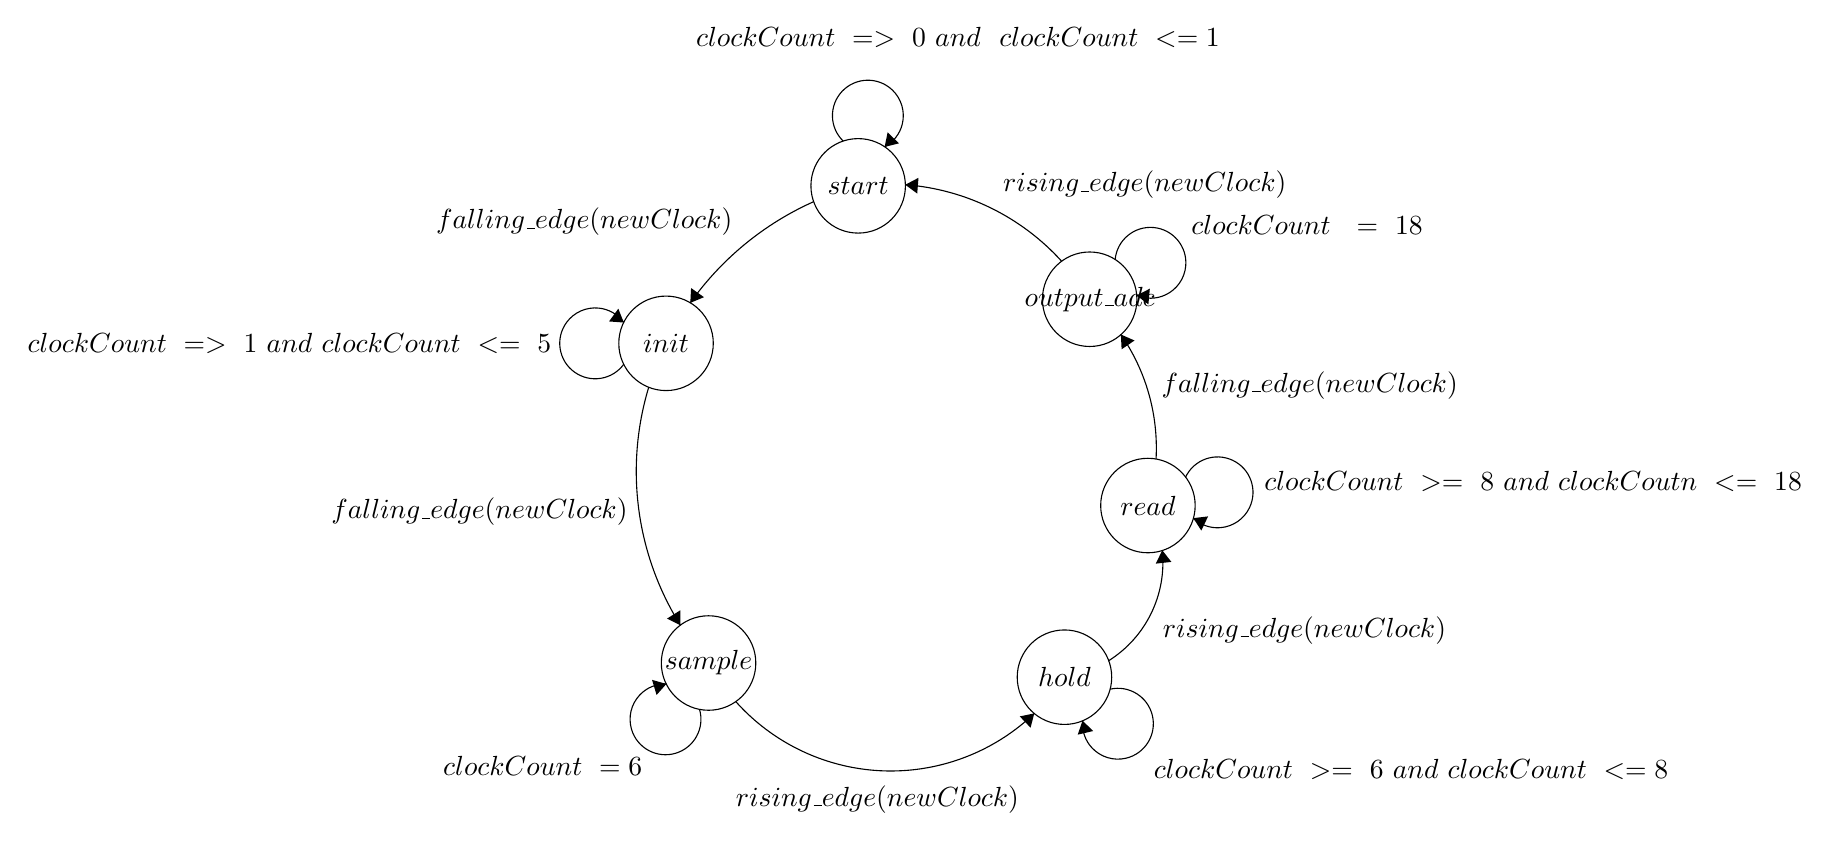
\begin{tikzpicture}[scale=0.2]
\tikzstyle{every node}+=[inner sep=0pt]
\draw [black] (36.2,-13.3) circle (3);
\draw (36.2,-13.3) node {$start$};
\draw [black] (24,-23.3) circle (3);
\draw (24,-23.3) node {$init$};
\draw [black] (26.7,-43.6) circle (3);
\draw (26.7,-43.6) node {$sample$};
\draw [black] (49.3,-44.5) circle (3);
\draw (49.3,-44.5) node {$hold$};
\draw [black] (54.6,-33.6) circle (3);
\draw (54.6,-33.6) node {$read$};
\draw [black] (50.9,-20.5) circle (3);
\draw (50.9,-20.5) node {$output\_adc$};
\draw [black] (35.257,-10.464) arc (226.1237:-61.8763:2.25);
\draw (42.54,-4.58) node [above] {$clockCount\mbox{ }=>\mbox{ }0\mbox{ }and\mbox{ }\mbox{ }clockCount\mbox{ }<=1$};
\fill [black] (37.88,-10.83) -- (38.79,-10.6) -- (38.07,-9.9);
\draw [black] (25.539,-20.728) arc (144.62852:114.05252:19.217);
\fill [black] (25.54,-20.73) -- (26.41,-20.37) -- (25.59,-19.79);
\draw (18.8,-16.5) node [above] {$falling\_edge(newClock)$};
\draw [black] (21.32,-24.623) arc (324:36:2.25);
\draw (16.75,-23.3) node [left] {$clockCount\mbox{ }=>\mbox{ }1\mbox{ }and\mbox{ }clockCount\mbox{ }<=\mbox{ }5$};
\fill [black] (21.32,-21.98) -- (20.97,-21.1) -- (20.38,-21.91);
\draw [black] (24.91,-41.197) arc (-147.98825:-196.85944:18.423);
\fill [black] (24.91,-41.2) -- (24.91,-40.25) -- (24.06,-40.78);
\draw (21.59,-34.01) node [left] {$falling\_edge(newClock)$};
\draw [black] (26.122,-46.532) arc (16.58935:-271.41065:2.25);
\draw (16.17,-49.46) node [below] {$clockCount\mbox{ }=6$};
\fill [black] (24.02,-44.93) -- (23.11,-44.67) -- (23.4,-45.63);
\draw [black] (47.385,-46.801) arc (-46.29147:-138.2695:13.191);
\fill [black] (47.38,-46.8) -- (46.46,-46.99) -- (47.15,-47.71);
\draw (37.42,-51.33) node [below] {$rising\_edge(newClock)$};
\draw [black] (52.189,-45.262) arc (102.95529:-185.04471:2.25);
\draw (54.94,-50.38) node [right] {$clockCount\mbox{ }>=\mbox{ }6\mbox{ }and\mbox{ }clockCount\mbox{ }<=8$};
\fill [black] (50.45,-47.26) -- (50.14,-48.15) -- (51.12,-47.92);
\draw [black] (55.509,-36.437) arc (6.09968:-57.96129:7.365);
\fill [black] (55.51,-36.44) -- (55.1,-37.29) -- (56.09,-37.18);
\draw (55.51,-41.52) node [right] {$rising\_edge(newClock)$};
\draw [black] (56.987,-31.802) arc (154.72166:-133.27834:2.25);
\draw (61.96,-32.06) node [right] {$clockCount\mbox{ }>=\mbox{ }8\mbox{ }and\mbox{ }clockCoutn\mbox{ }<=\mbox{ }18$};
\fill [black] (57.48,-34.4) -- (57.99,-35.19) -- (58.42,-34.29);
\draw [black] (52.882,-22.743) arc (34.69202:-3.14813:12.673);
\fill [black] (52.88,-22.74) -- (52.93,-23.68) -- (53.75,-23.12);
\draw (55.43,-25.96) node [right] {$falling\_edge(newClock)$};
\draw [black] (39.194,-13.226) arc (85.64928:42.15987:14.921);
\fill [black] (39.19,-13.23) -- (39.95,-13.79) -- (40.03,-12.79);
\draw (54.4,-14.15) node [above] {$rising\_edge(newClock)$};
\draw [black] (52.518,-17.988) arc (174.93908:-113.06092:2.25);
\draw (57.33,-15.77) node [right] {$clockCount\mbox{ }\mbox{ }=\mbox{ }18$};
\fill [black] (53.88,-20.26) -- (54.63,-20.83) -- (54.72,-19.83);
\end{tikzpicture}
\end{turn}
\end{document}
